\documentclass{article}
\usepackage[UTF8]{ctex}
\usepackage[tc]{titlepic}
\usepackage{titlesec}
\usepackage{cite}
\usepackage{amsmath}
\usepackage{fancyhdr}
\usepackage{booktabs}
\usepackage{graphicx}
\usepackage{geometry}
\usepackage[section]{placeins}
\geometry{a4paper,scale=0.8}
\pagestyle{fancy}

\lhead{第一次作业\\\today}
\chead{中国科学技术大学\\数学建模课程}

\rhead{Assignment x\\ {\CTEXoptions[today=old]\today}}
\newcommand{\upcite}[1]{\textsuperscript{\cite{#1}}}

\titleformat*{\section}{\bfseries\Large}
\titleformat*{\subsection}{\bfseries\large}

\title{\bfseries 接缝裁剪的图像缩放}
\author{时分 \quad  999 \quad  PB23151799}

\begin{document}
\maketitle
\begin{abstract}
    为解决传统图像缩放方法导致的图像完整度下降和关键信息丢失问题，本报告介绍了一种具有保持原图像完整度能力的图像裁剪方法————接缝裁剪（Seam Carving），描述了基于拉普拉斯算子的图像卷积算法、能量矩阵的计算和基于动态规划寻找缝隙的数学建模原理。在MATLAB环境下完成了代码实现，将其应用于两张示例图像的缩放。最后，从算法设计和时间复杂度优化的角度，提出了一些可以改进的问题。
\end{abstract}
\clearpage
% \setcounter{secnumdepth}{1}
 \setcounter{section}{1}
\section*{\centerline{一、前言}}
    图像缩放（image scaling）是指对数字图像的大小进行调整的过程，包括图像放大和图像缩小。常见的图像缩小算法，如基于等间隔采样的图像缩小算法、基于局部均值的图像缩小算法等，虽然可以有效地缩小图像，但由于缺乏对图像内容的分析，这些算法会缺乏选择性地将图像各个部分进行压缩，对图像关键信息的完整性造成了破坏\upcite{Brook2014}。同时，当缩小后长宽比例与原图像不同时，这些算法往往还会导致图像内容的扭曲变形。为解决这些问题，Shai Avidan和Ariel Shamir提出了一种内容感知图像缩放算法，即接缝裁剪（Seam Carving）算法\upcite{Avidan2007}，它具有如下的特征：
    \begin{itemize}
      \item 可以有效地将图像按任意尺寸比例缩小；
      \item 可以有效地保留图像的主要部分与关键信息；
      \item 避免让图像内容扭曲变形。
    \end{itemize}\
    由于具有这些特征，接缝裁剪算法为图像缩放提供了一个更“智能”的方法，可以更好地适用于部分图像，如风景照片、静物照片的缩放情境。
 \setcounter{section}{2}
\section*{\centerline{二、问题分析}}
    接缝裁剪算法应用于图像缩小时，需要解决如下几个问题：
    \begin{enumerate}
      \item 如何感知图像的内容？
      \item 如何量化图像像素的关键程度？
      \item 如何确定要移除的像素？以什么方式移除像素？
    \end{enumerate}
    
    为感知图像内容，本报告的算法实现采取了拉普拉斯算子的卷积核，对图像进行滤波，从而同时捕捉像素在横向、纵向的变化量大小（偏导）。同时，引入能量函数量化像素的能量大小，即衡量像素的“关键程度”。
    
    算法希望找到一条“缝隙”（seam），这条缝隙由上至下或由左至右，每两个相邻的像素间行、列间距不超过1，并使得缝隙中的像素点能量之和尽可能小。本报告采取动态规划的方法，从上向下寻找一条能量总和较小的缝隙并将其从图像中移除，重复该过程多次以达成缩小图像的效果。
 \setcounter{section}{3}
\section*{\centerline{三、数学模型建立}}
    首先，用拉普拉斯算子对图像进行滤波，卷积核为
    \[\begin{bmatrix}
      0.5 & 1 & 0.5 \\
      1 & -6 & 1 \\
      0.5 & 1 & 0.5 
    \end{bmatrix}\]
    
    对滤波后的图像\(\mathbf{F}_{r \times c \times 3}\)，引入能量函数
    \[\mathbf{G}(i,j) = cost(\mathbf{F}(i,j)) = \sum_{3}^{k=1}  \mathbf{F}(i,j,k)^2\]
    其中\(\mathbf{G}_{r \times c}\)为图像的能量矩阵，\(\mathbf{F}_{r \times c \times 3}\)的第三维度为RGB三通道，\(r,c\)分别为图像像素的行数、列数。
    
    之后采取动态规划的方法，引入矩阵\(\mathbf{M}_{r \times c}\)，其中
    \begin{equation*}
    \mathbf{M}(i,j) = 
    \begin{cases}
    \mathbf{G}(i,j),i=1,1<=j<=c \\
    \mathbf{G}(i,j) + min\{\mathbf{M}(i-1,j),\mathbf{M}(i-1,j+1)\},2<=i<=r,j=1 \\
    \mathbf{G}(i,j) + min\{\mathbf{M}(i-1,j-1),\mathbf{M}(i-1,j),\mathbf{M}(i-1,j+1)\},2<=i<=r,2<=j<=c-1 \\
    \mathbf{G}(i,j) + min\{\mathbf{M}(i-1,j-1),\mathbf{M}(i-1,j)\},2<=i<=r,j=c
    \end{cases}
    \end{equation*}
    \(\mathbf{M}\)的最后一行表示了各路径的能量之和，最后一行的最小值即指示了能量较低的缝隙。
    
    算法接下来删除该条缝隙上的所有像素，得到列数减少一的新图像。重复该过程裁剪列数，结合90度旋转操作以裁剪行数，即可得到按任意尺寸缩小的图像。
 \setcounter{section}{4}
\section*{\centerline{四、结果}}
    采用图片peppers.png，图像尺寸为384*512,RGB三通道，利用接缝裁剪算法将其裁剪为384*462的新图像，效果如图1。
    \begin{figure}[h]
        \centering %居中
        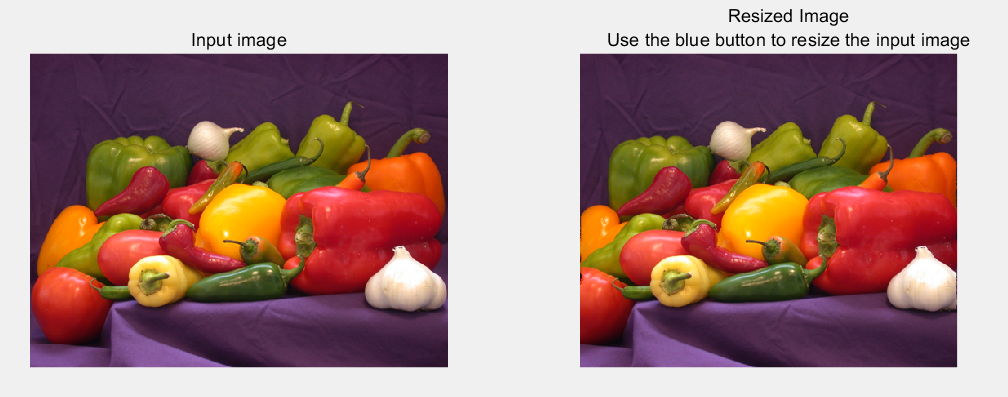
\includegraphics[scale=0.5]{Result_Peppers.png}
        \caption{使用接缝裁剪算法缩小peppers.png的结果}
    \end{figure}
    
    采用图片YexiLake.png，图像尺寸为666*422,RGB三通道，利用接缝裁剪算法将其裁剪为666*322的新图像，效果如图2。
    \begin{figure}[h]
        \centering %居中
        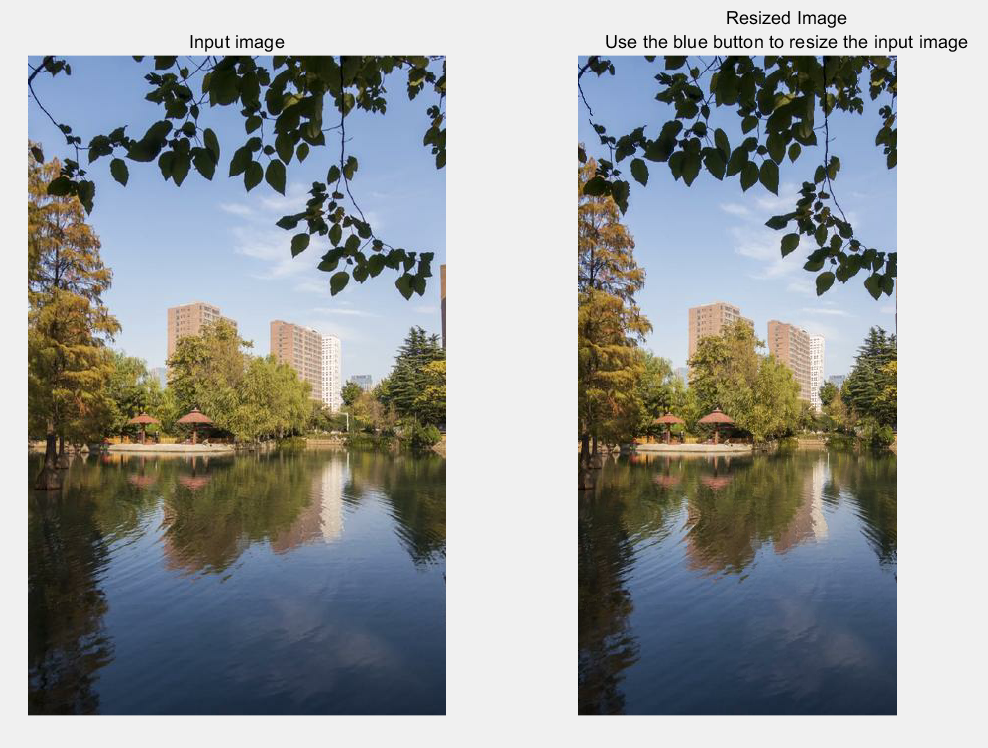
\includegraphics[scale=0.5]{Result_YexiLake.png}
        \caption{使用接缝裁剪算法缩小YexiLake.png的结果}
    \end{figure}
    
    本报告实现的接缝裁剪算法保留了图像的关键部分，在不破坏图像完整性的情况下，在完成两张图像的缩小任务中均表现出较好的效果。
 \setcounter{section}{5}
\section*{\centerline{五、结论}}
    本报告中的接缝算法通过基于拉普拉斯算子的图像卷积算法对图像进行分析，计算出能量矩阵之后，通过动态规划选出能量较小的缝隙并删除，并在测试图像中表现出良好的效果。

 \setcounter{section}{6}
\section*{\centerline{六、问题}}
    \subsection{寻找缝隙的其他算法}
    本报告中的算法基于动态规划的思想寻找能量较小的缝隙，对图像\(\mathbf{F}_{r \times c \times 3}\)获取了与最后一排像素一一对应的\(c\)条路径。

    考察缝隙的定义，我们发现这一过程也可以从图的角度加以解释。把图像建模为一张有向图，每个像素可以看作一个顶点。该顶点前后分别有3个像素、共6个像素与其由有向边连接，由前排像素指向后排，权重为边尾的像素能量值。在这一建模下，寻找缝隙的过程可以看作从第一排像素出发，在有向图中寻找最短路径的过程，从而可以应用Dijkstra算法等寻找最短路径的算法。

    \subsection{时间复杂度的优化}
    对图像\(\mathbf{F}_{r \times c \times 3}\)，本报告中的寻找能量最小缝隙的算法时间复杂度为\(O(r \times c)\)，在删除每条缝隙中调用一次，若需要删除\(q\)条缝隙，则总的时间复杂度为\(O(r \times c \times q)\)。

    基于时间复杂度较高的问题，本报告提出两种可能的改进方案：
    \begin{itemize}
        \item 基于动态规划的思想，每次寻找\(h\)条能量最低的缝隙（这一步长可以调整，理论上步长越短，效果越好）；按能量从低到高排列，按顺序删除其中没有交叉的所有缝隙；重复这一过程直到删除\(q\)条缝隙为止。这一算法最劣情况的时间复杂度为\(O(r \times c \times q)\)，通常情况下会优于本报告中的算法。
        \item 基于动态规划的思想，一次寻找\(q\)条能量最低的缝隙对应的最后一排\(q\)个像素；按能量从低到高排列，从这\(q\)个像素出发，逐个删除包含它们的能量最低缝隙（逐个删除可以保证删除的像素不重复）。
    \end{itemize}
    
    这两种改进方案都可以较显著地改善算法的时间复杂度，但也不可避免地降低了裁剪的精度。在处理分辨率较高的图像时，这两种改进方案具有较好的效果。
\bibliographystyle{ieeetr}
\bibliography{refer}

\end{document} 